\chapter{SAF microarchitecture primitive taxonomy}
\label{chapter:primitive_taxo_model}

This section introduces a taxonomy of SAF microarchitecture primitives. Each taxonomic primitive expresses a basic operation that is key to implementing sparse tensor arithmetic, staying as close as possible to the \textit{Efficient Processing}\cite{szebook} taxonomy. 

The taxonomic system in this work is modeled off of C++ generics: 

\begin{itemize}
    \item This work defines a number of \textbf{taxonomic category templates} (or just \textit{categories}), which are analogous to \textit{C++ templates}. A taxonomic category in this work is parameterized by a set of \textbf{attributes}, which are analogous to \textit{template parameters} in C++ templates.
    \item A taxonomic category in this work is \textit{customized} by specifying attribute values, just as a \textit{C++ template customization} is the result of invoking a C++ template and specifying all of the template parameters. In this work, all possible legal combinations of attribute values for a given taxonomic category are referred to as the \textit{supported customizations} or just \textit{customizations} for that category.
    \item Within a given taxonomic category, there is \textbf{complete flexibility to adjust the primitive's RTL blocks, scale parameters, and constitutive relations for each customization}.
    \item To \textit{instantiate} a taxonomic primitive, is to realize a specific occurrence of the customized primitive within some design. \textit{Instantiation} in this work is analogous to \textit{instantiating} an object by calling the constructor for a particular template customization of a C++ class. In this work, instantiation is not possible unless all primitive attributes have been specified, i.e. a single customization has been unambiguously specified.
\end{itemize}

Conceptually, the taxonomic category describes a format-agnostic and broadly context-agnostic SAF microarchitecture primitive, while the category's customizations reflect that the primitive implementation is interdependent on format and characteristics of the surrounding design. This accomplishes the goal of keeping the taxonomy as format- and generally context-agnostic as possible (as discussed in Chapter~\ref{chapter:conceptual_framework} and also in \textit{Efficient Processing}\cite{szebook}); at the same time, the customizations make it easy to consider a primitive's more detailed implementation when it is necessary or helpful.

In addition to its taxonomic attributes, each SAF microarchitecture primitive is associated with:

\begin{itemize}
    \item \textbf{An interface}, comprising input and output ports. Each port has one of three \textit{Efficient Processing} interface types: \textit{metadata format}, \textit{position}, or \textit{flag}.
    \item \textbf{An analytical energy/area/timing model}, which is parameterized by the primitive's attributes.
\end{itemize}

By pairing each taxonomic primitive with an analytical model, we accomplish the goal described in Chapter~\ref{chapter:conceptual_framework} of evaluating and comparing designs.

In order to stay as close to the \textit{Efficient Processing} taxonomy as possible, it is desirable that the primitive's input and output ports can be understood as transmitting/receiving metadata, position or flag values. The ideal SAF microarchitecture primitive is domain-specific to tensor acceleration. Thus, SAF microarchitecture primitives are \textit{not} synonymous with RTL blocks from Chapter~\ref{chapter:rtl}, because RTL blocks are not \textit{necessarily} domain-specific in the way that SAF microarchitecture primitives are. A SAF microarchitecture primitive is constructed from zero or more RTL blocks.

In this work, the following rules are followed when deciding which SAF microarchitecture primitive characteristics should be captured as taxonomic attributes, versus which characteristics should be captured as scale parameters:

\begin{itemize}
    \item \textbf{Does the characteristic in question distinguish paradigmatically different approaches to implementing the primitive functionality?} Example: tree vs ripple implementation is a good candidate for a taxonomic attribute. Counter-example: most low-level pipelining decisions, unless they impact scaling behavior, should be scaling parameters in the primitive model, if they are even represented at all.
    \item \textbf{Does the characteristic in question impact the \textit{shape of the component's scaling trend}?} Example: pipelining a multi-step operation over multiple pipeline stages, versus combinationally unrolling multiple iterations of the operation within a single pipeline stage; this distinction is a good candidate for a taxonomic attribute since it strongly impacts the scaling behavior of propagation delay, and by extension the feasibility of the design. Counter-example: the particular choice of metadata word bitwidth does not change the \textit{shape} of the primitive's scaling behavior, however it \textit{does} select a particular point on the scaling curve, and so is an excellent candidate for a scaling parameter.
\end{itemize}

The following sections will introduce the SAF microarchitecture primitive categories developed for this work. 

For brevity, the analytical model definitions will not be provided for the primitives in this section. However, the transfer relation model for coordinate-payload intersection, developed in Section~\ref{sec:c_c_isect_modeling}, is an example of how to go about building analytical models of SAF microarchitecture primitives.

\section{Metadata parser taxonomic category template}

\begin{figure}[H]
    \centering
    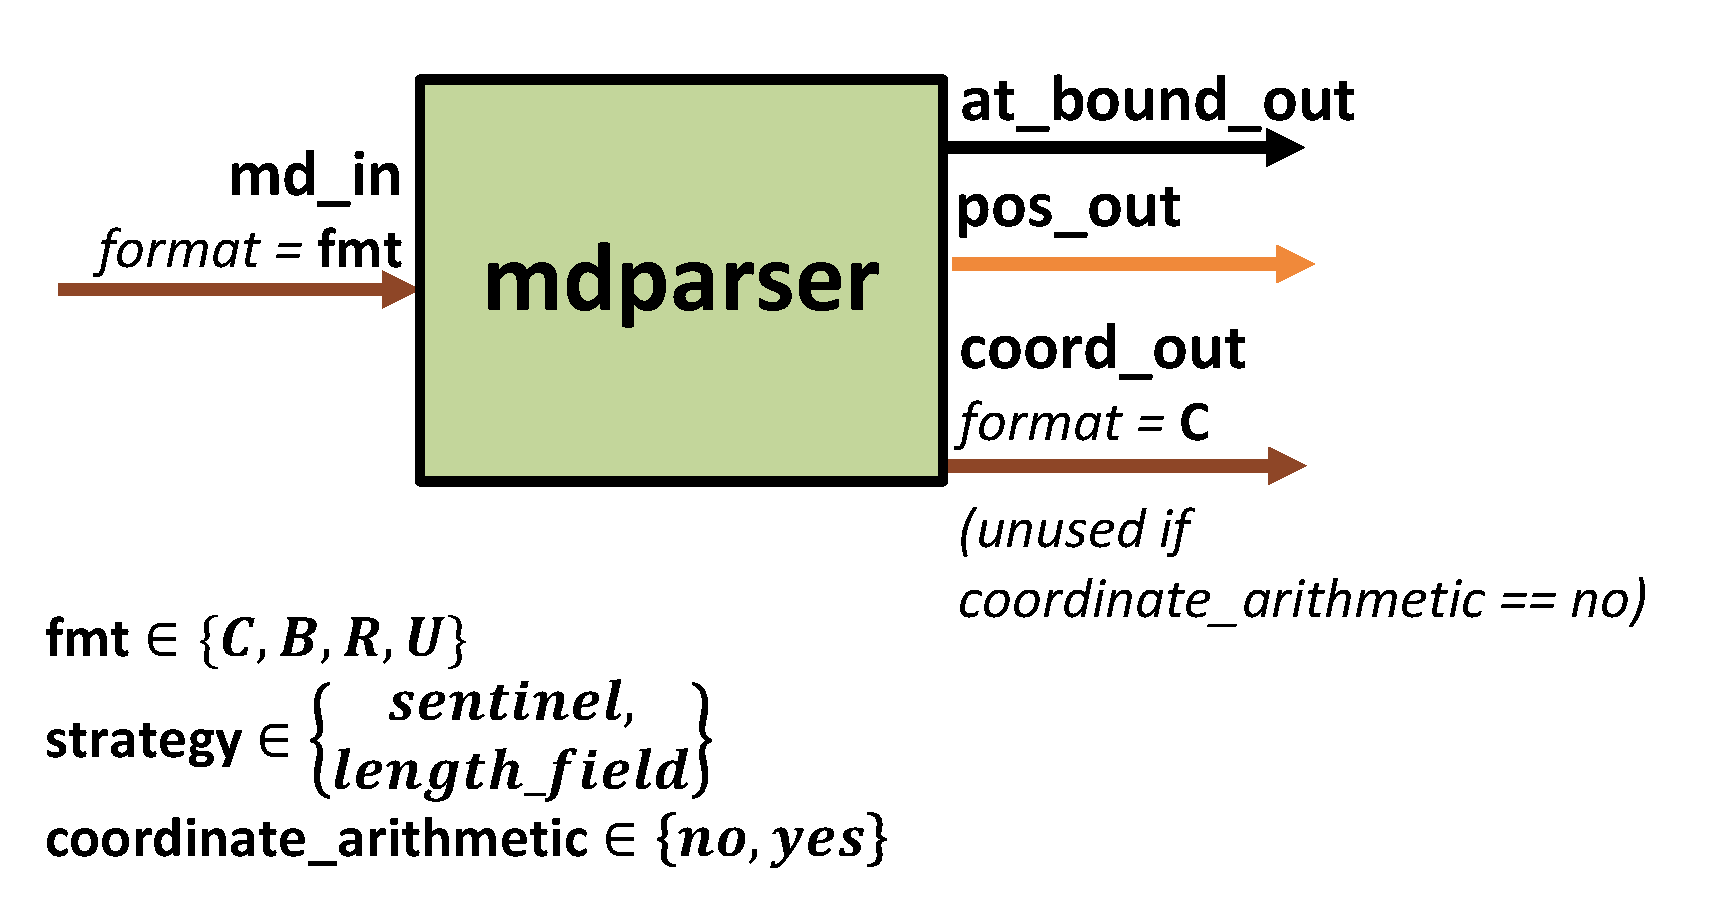
\includegraphics[width=0.95\textwidth]{figures/mdparser.pdf}
    \caption{Metadata parser primitive component template.}
    \label{fig:mdparser}
\end{figure}

The metadata parser SAF microarchitecture primitive (mdparser) follows the functionality described in Section~\ref{chapter:conceptual_framework}, parsing sparse format metadata and outputting (1) positional offsets for looking up payloads (\textit{pos\_out}) and (2) reset signals at the end of fiber traversal (\textit{at\_bound\_out}.) Additionally, for implicit coordinate formats, the metadata parser can \textit{optionally} compute explicit coordinates to support coordinate coordinate computation.

The metadata parser primitive attributes are

\begin{itemize}
    \item \textbf{format -} The sparse representation format supported by the metadata parser.
    \item \textbf{strategy -} The strategy employed by the metadata parser for detecting the end of traversal.
    \begin{itemize}
        \item \textbf{sentinel -} a sentinel symbol is detected at the end of the fiber (depending on the format, the symbol may appear at the end of the metadata, or at the end of the fiber payload array.)
        \item \textbf{length\_field -} the fiber metadata includes a value which is the length of the fiber (depending on the format, this may be the length of the metadata array, or the length of the payload array.)
    \end{itemize}
    \item \textbf{coordinate\_arithmetic -} \textit{yes} if the metadata parser must compute explicit coordinates, \textit{no} otherwise.
\end{itemize}

The supported metadata parser specializations are shown in Table~\ref{tab:MetadataParser_specializations}.

\begin{table}[H]
\centering
\begin{tabular}{lll}
\toprule
 format   & strategy       & coordinate\_arithmetic   \\
\midrule
 U        & sentinel & no\_arithmetic                \\
 U        & sentinel & yes\_arithmetic                 \\
 U        & length\_field & no\_arithmetic              \\
 U        & length\_field & yes\_arithmetic             \\
 C        & sentinel & no\_arithmetic                \\
 C        & sentinel & yes\_arithmetic                 \\
 C        & length\_field & no\_arithmetic              \\
 C        & length\_field & yes\_arithmetic             \\
 B        & sentinel & no\_arithmetic                  \\
 B        & sentinel & yes\_arithmetic                 \\
 B        & length\_field & no\_arithmetic              \\
 B        & length\_field & yes\_arithmetic             \\
\bottomrule
\end{tabular}
\caption{Specializations of metadata parsers.}
\label{tab:MetadataParser_specializations}
\end{table}

\section{Coupled position generators}

Recall from Section~\ref{chapter:conceptual_framework} that \textit{coupled} position generators output position offsets in payload memory, conditional on metadata values provided as input. Thus coupled position generators are classified as SAF microarchitecture.

\subsection{Single position generator taxonomic category template}

\begin{figure}[H]
    \centering
    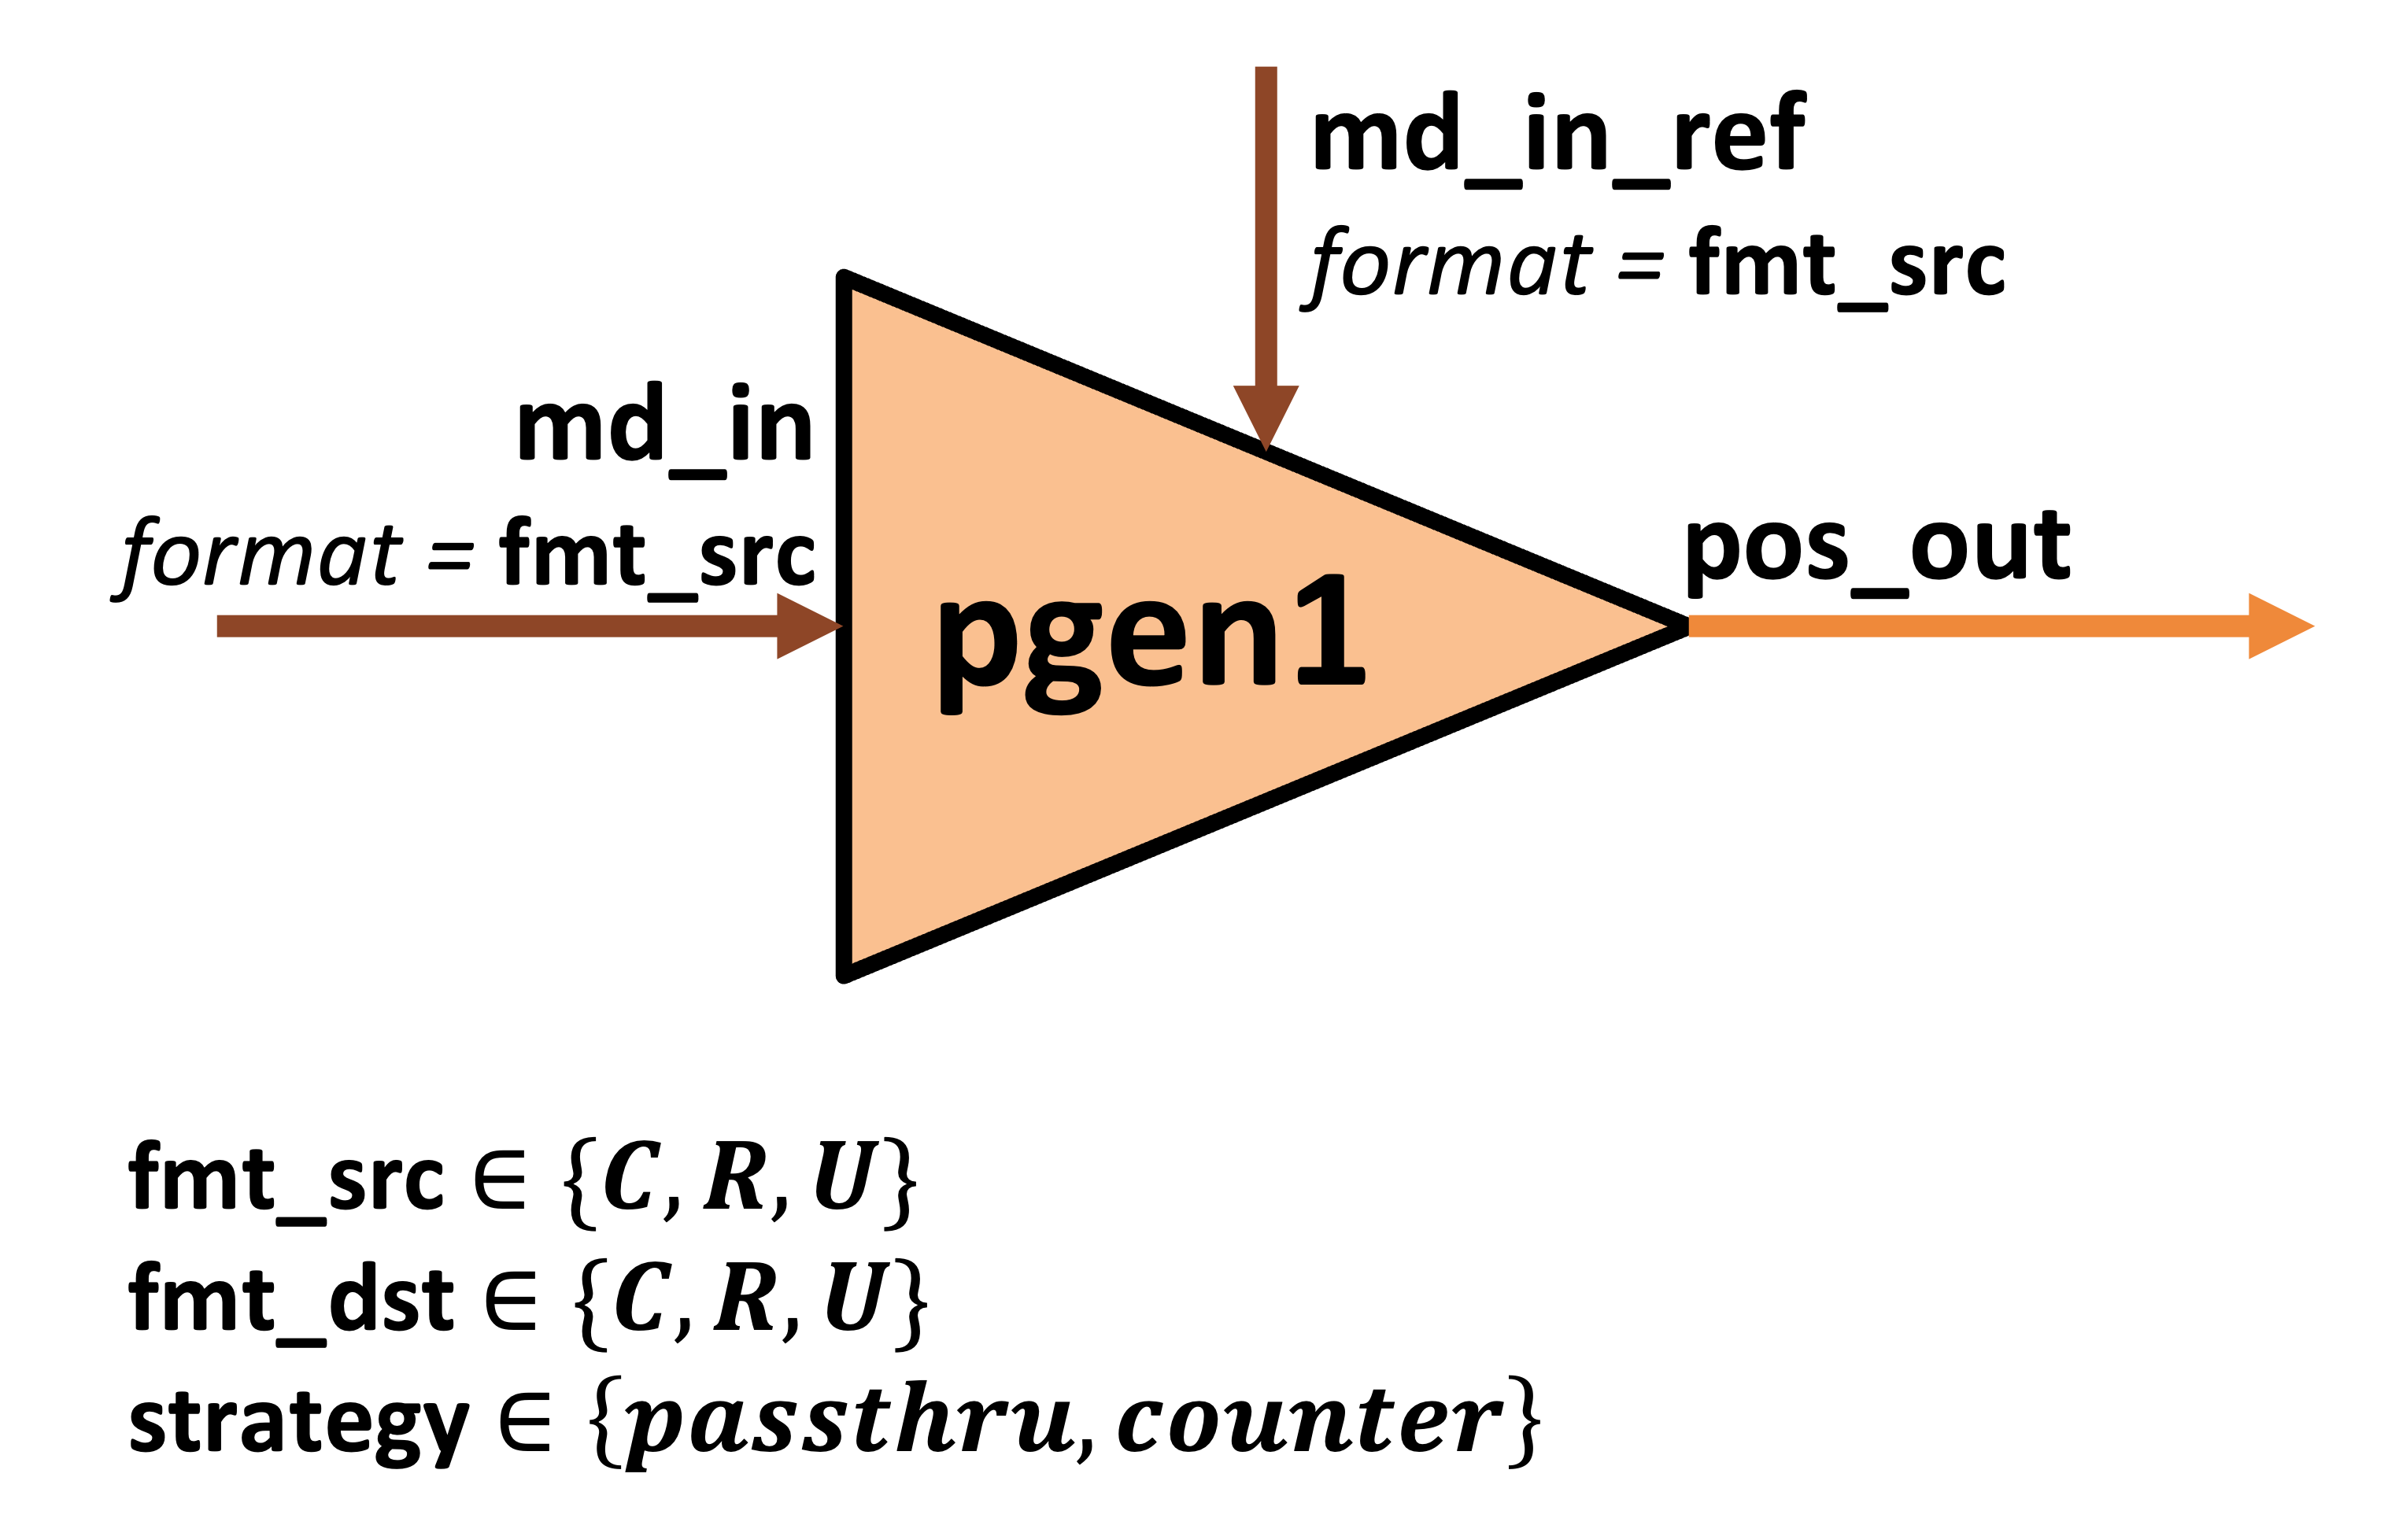
\includegraphics[width=0.95\textwidth]{figures/pgen1.png}
    \caption{Single position generator primitive component template.}
    \label{fig:pgen1}
\end{figure}

The Single position generator (pgen1, Figure~\ref{fig:pgen1}) converts a single metadata input stream into a single position offset output stream. It is used, for example, in coordinate-payload bidirectional skipping microarchitectures, as described in Section~\ref{chapter:conceptual_framework}.

Depending on the particular customization (i.e. the \textit{counter}-based strategy), the pgen1 may exploit the reference input (\textit{md\_in\_ref}), computing positional offsets based on comparing the primary metadata input to the reference input.

However, the \textit{passthrough} strategy is simply a wire directly from the primary metadata input to the position output, so the reference input is not utilized for this strategy.

Which strategies are valid, is dependent on (1) the format of the input metadata and (2) the format of the fiber which the position offsets will index into. The pgen1 has the following attributes:

\begin{itemize}
    \item \textbf{format\_src -} The format of the ``source'' fiber which originates the metadata input.
    \item \textbf{format\_dst -} The format of the ``destination'' fiber, which the positional offsets generated at the output will index into.
    \item \textbf{strategy -} The approach to implementing position offset generation. Strongly influences whether and how the reference input is utilized.
    \begin{itemize}
        \item \textbf{passthrough -} Wire directly from primary metadata input to position output; reference input is not utilized.
        \item \textbf{counter -} Each metadata value arriving at the reference input increments a counter (the amount of increment is equal to the input vectorization of the pgen1 unit, which is a lower-level scale parameter.) When a metadata value arrives at the primary input, the pgen1 outputs the counter value. This represents the scenario in which the primary input is connected to an coordinate-payload intersection unit's output, and the reference input is connected to one of the skipping microarchitecture's input metadata streams; the output position offsets represent the index of the matching metadata values, within the particular input metadata stream.
    \end{itemize}
\end{itemize}

Single position generator specializations are shown in Table~\ref{tab:SinglePositionGenerator_specializations}.

\begin{table}[H]
\centering
\begin{tabular}{lll}
\toprule
 format\_src   & format\_dst   & strategy    \\
\midrule
 C            & U            & passthrough \\
 C            & C            & counter     \\
\bottomrule
\end{tabular}
\caption{Specializations of Single position-generator}
\label{tab:SinglePositionGenerator_specializations}
\end{table}

\subsection{Dual position generator taxonomic category template}

\begin{figure}[H]
    \centering
    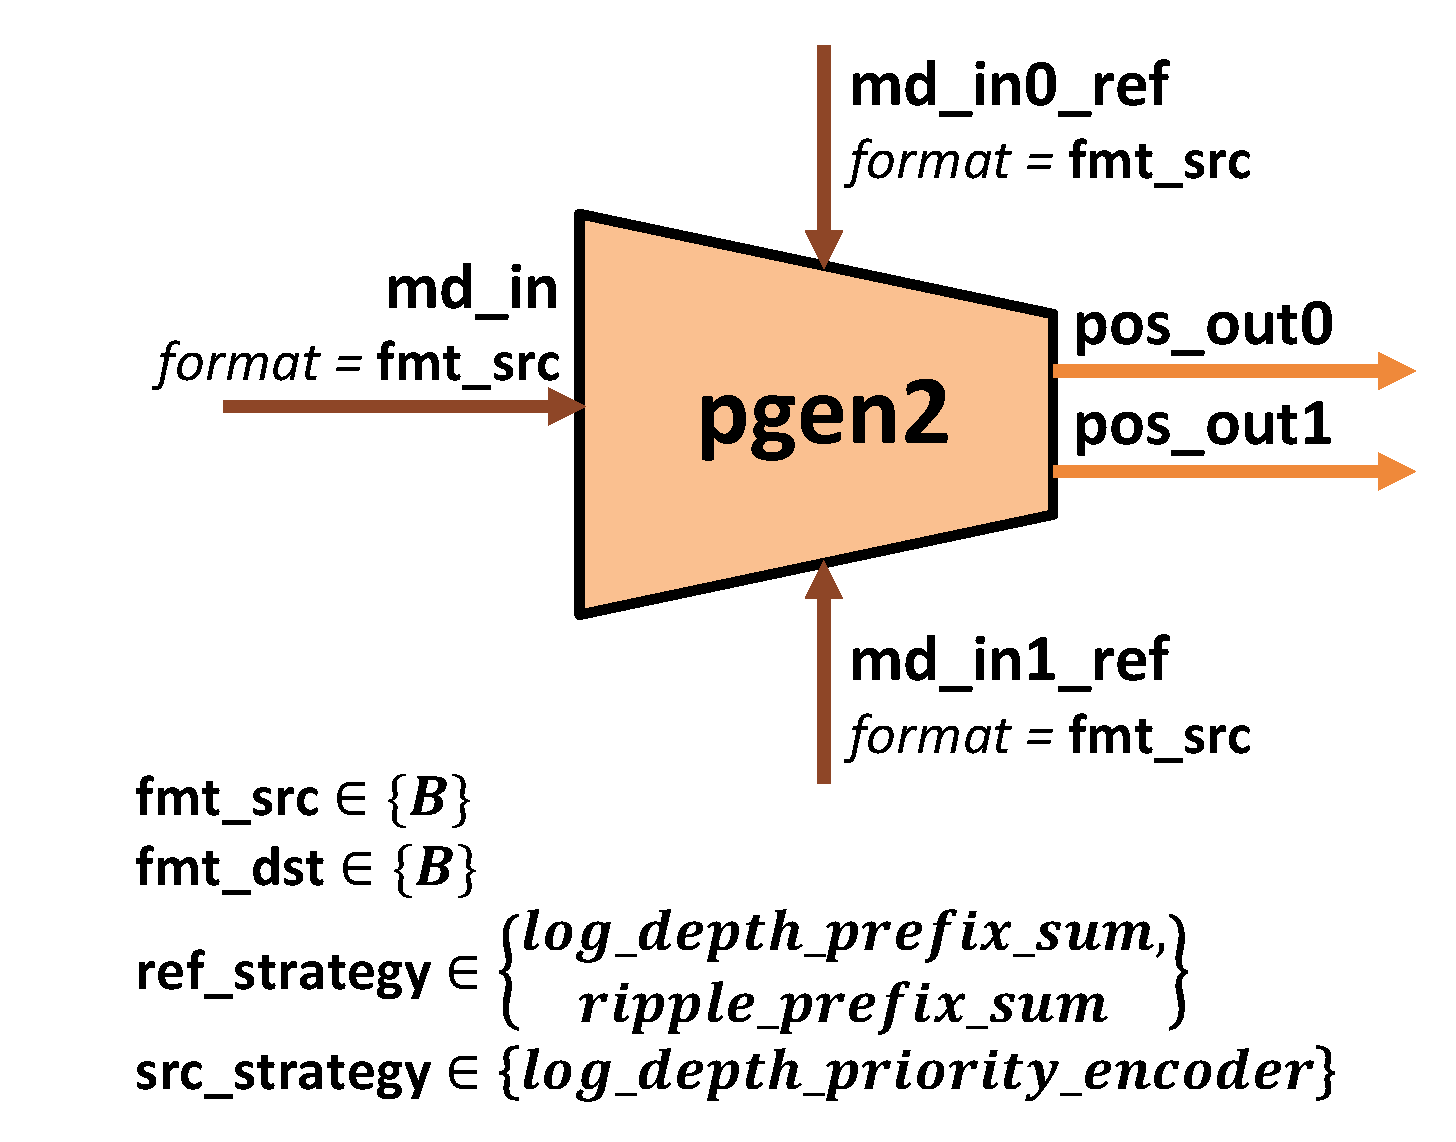
\includegraphics[width=0.95\textwidth]{figures/pgen2.pdf}
    \caption{Dual position generator primitive component template.}
    \label{fig:pgen2}
\end{figure}

The Dual position generator (pgen2, Figure~\ref{fig:pgen2}) converts a single metadata input stream into a two position offset output streams. pgen2 is utilized, for example, in bitmask intersection units, as described in Section~\ref{chapter:conceptual_framework}.

Like pgen1, pgen2 has a single metadata input; unlike pgen1, pgen2 has two reference inputs and two positional offset outputs. 

pgen2 compares the primary metadata input, to both of the reference inputs; the comparison to the first reference input yields the first position offset output stream, and the comparison to the second reference input yields the second position offset output stream.

pgen2 assumes that all metadata inputs are sourced from fibers of the same representation format, and that both positional outputs are indexing into fibers with the same representation format.

The pgen2 has the following attributes -

\begin{itemize}
    \item \textbf{format\_src -} The format of the ``source'' fibers which originate the metadata inputs.
    \item \textbf{format\_dst -} The format of the ``destination'' fibers, which the positional offsets generated at the output will index into.
    \item \textbf{reference\_strategy -} The strategy for processing the reference metadata inputs. When format\_src is Bitmask (B), then reference\_strategy reflects the choice of RTL block used for computing prefix-sum of the reference metadata input streams. The options are:
    \begin{itemize}
        \item \textbf{ripple\_prefix\_sum }
        \item \textbf{kogge\_stone\_prefix\_sum}
    \end{itemize}
    These options refer to prefix-sum RTL blocks in Section~\ref{chapter:rtl}.
    \item \textbf{source\_strategy -} The strategy for processing the primary metadata input. If format\_src is Bitmask (B), then source\_strategy reflects the choice of RTL block used for priority encoder. The options are
    \begin{itemize}
        \item \textbf{parallel\_dec2\_priority\_encoder }
        \item A ripple priority encoder option would be interesting to explore but was not investigated in this work.
    \end{itemize}
\end{itemize}

Dual position generator specializations are shown in Table~\ref{tab:DualPositionGenerator_specializations}.

\begin{table}[H]
\centering
\begin{tabular}{llll}
\toprule
 format\_src   & format\_dst   & reference\_strategy        & source\_strategy             \\
\midrule
 B            & B            & ripple\_prefix\_sum      & parallel\_dec2\_priority\_encoder \\
 B            & B            & kogge\_stone\_prefix\_sum & parallel\_dec2\_priority\_encoder \\
\bottomrule
\end{tabular}
\caption{Specializations of dual position generator}
\label{tab:DualPositionGenerator_specializations}
\end{table}

\section{Intersection units}

Intersection units intersect two fibers and output a stream of metadata representing matches. The meaning of the match stream reflects the type of join being performed.

\subsection{Leader-follower intersection unit taxonomic category template}

The \textit{md\_in\_leader} input is the sparse metadata associated with the leader operand; the \textit{md\_out} output produces a stream of metadata corresponding to matches; see Figure~\ref{fig:isectlf}.

Leader-follower intersections perform a left-outer join between two fibers; thus, the output match stream reflects \textit{all} of the leader metadata, but only that follower metadata which matches the leader.

\begin{figure}[H]
    \centering
    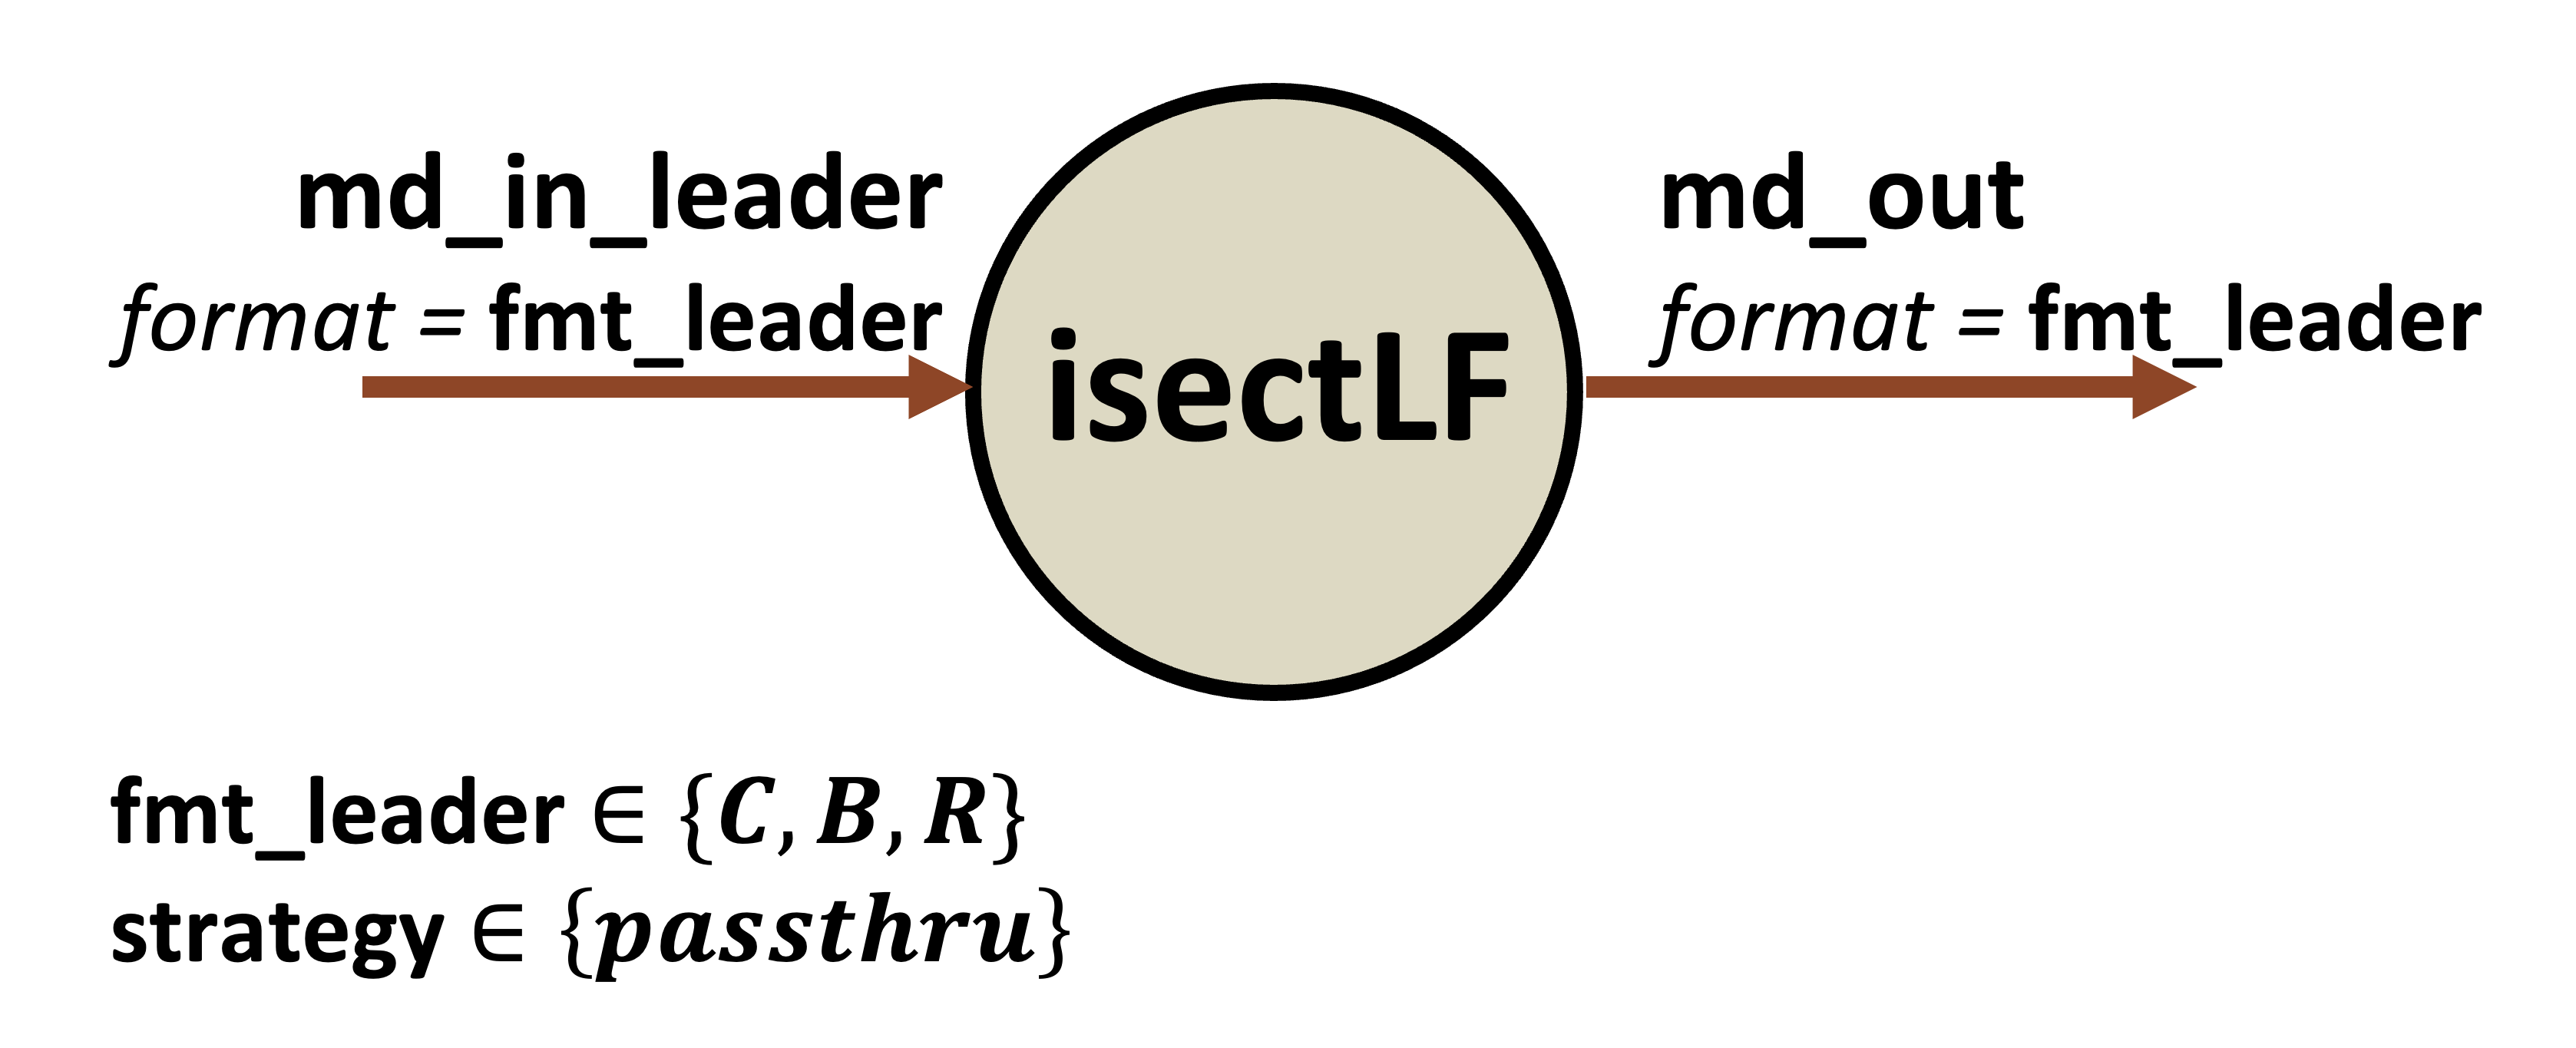
\includegraphics[width=0.95\textwidth]{figures/isectlf.png}
    \caption{Leader-follower intersection primitive component template.}
    \label{fig:isectlf}
\end{figure}

The leader-follower intersection SAF microarchitecture primitive attributes are:

\begin{itemize}
    \item \textbf{format\_leader -} The leader fiber sparse representation format.
    \item \textbf{strategy -} All leader-follower intersections implement a \textit{passthrough} strategy, i.e. a wire directly from input to output.
\end{itemize}

The supported customizations for leader-follower intersection are shown in Table~\ref{tab:IntersectionLeaderFollower_specializations}.

\begin{table}[H]
\centering
\begin{tabular}{ll}
\toprule
 format\_leader   & strategy    \\
\midrule
 C               & passthrough \\
 B               & passthrough \\
\bottomrule
\end{tabular}
\caption{Specializations of leader-follower intersection.}
\label{tab:IntersectionLeaderFollower_specializations}
\end{table}

\subsection{Bidirectional intersection unit taxonomic category template}

For bidirectional intersection unit, the \textit{md\_in0} and \textit{md\_in1} inputs receive sparse format metadata from the two fibers being intersected; the \textit{md\_out} output produces a stream of metadata corresponding to matches; see Figure~\ref{fig:isectbd}.

Bidirectional intersections perform an inner join between two fibers; thus, the output match stream reflects \textit{only} the metadata for coordinates which are common to both fibers.

\begin{figure}[H]
    \centering
    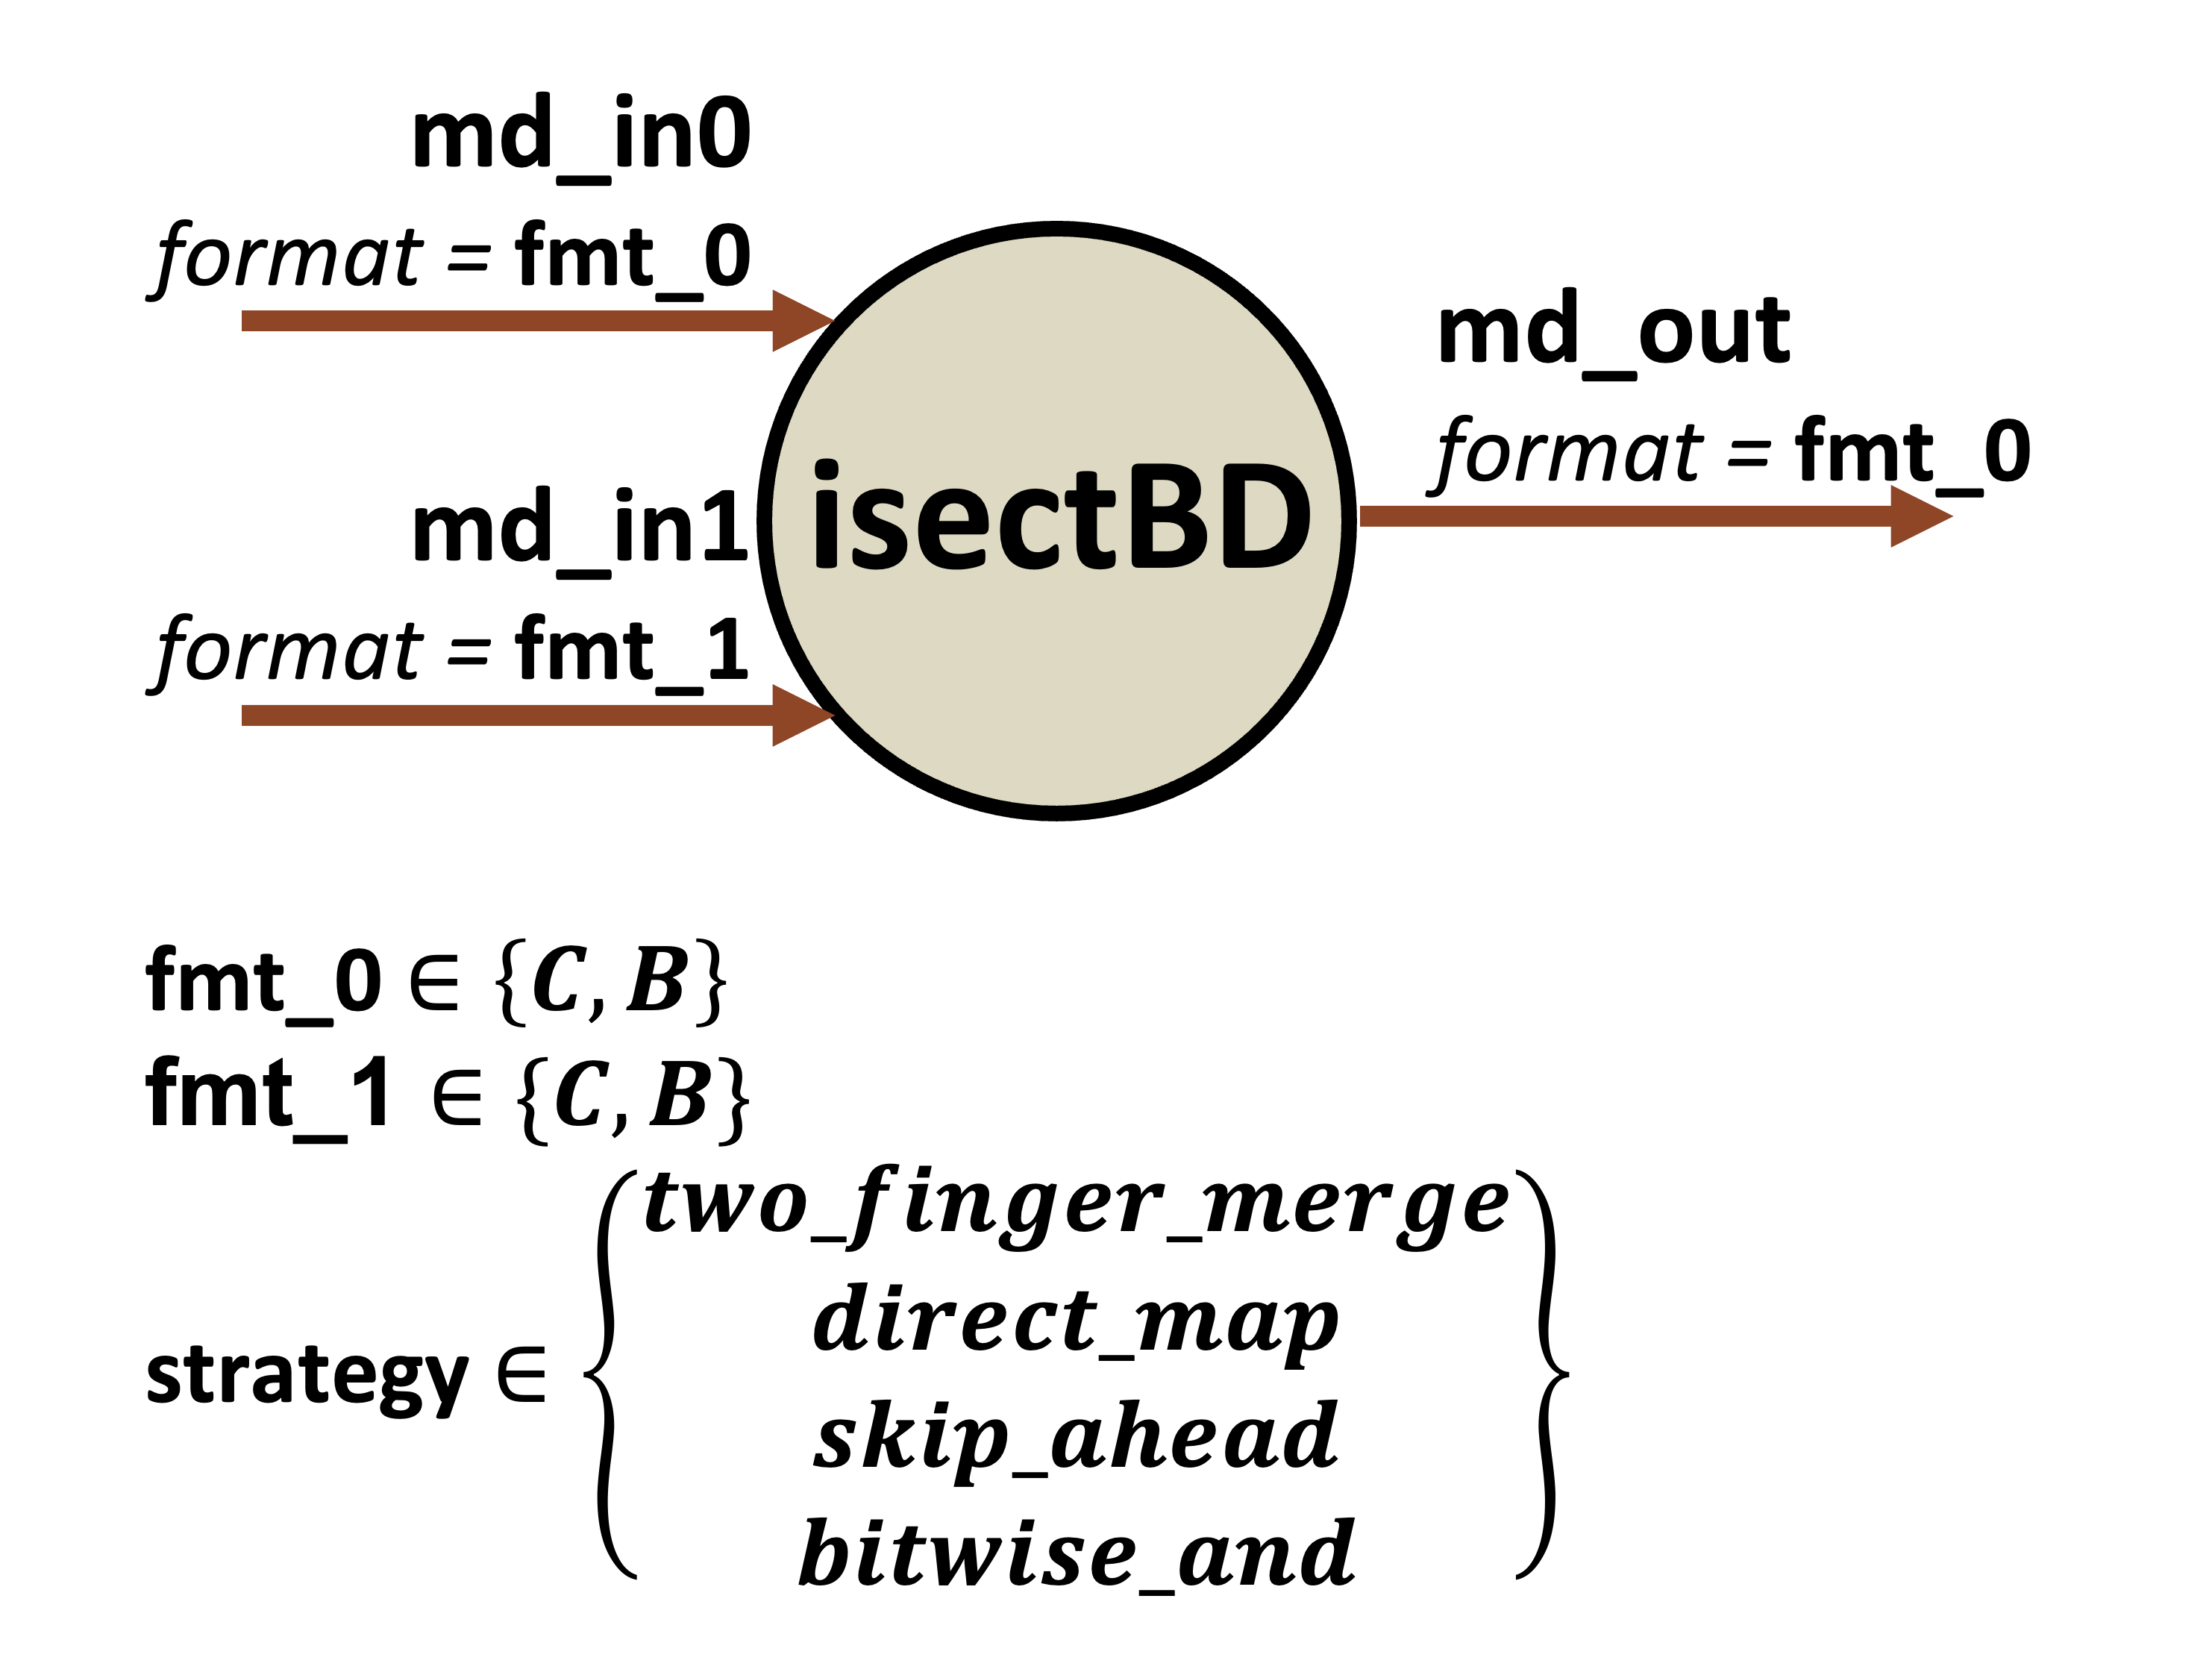
\includegraphics[width=0.95\textwidth]{figures/isectbd.png}
    \caption{Bidirectional intersection primitive component template.}
    \label{fig:isectbd}
\end{figure}

The attributes of a bidirectional intersection unit are

\begin{itemize}
    \item \textbf{format\_0}, \textbf{format\_1 -} The formats of the two input fibers being intersected.
    \item \textbf{strategy -} The approach to implementing bidirectional intersection. \textit{strategy} is effectively selecting an intersection unit RTL block from Section~\ref{chapter:rtl}.
    \begin{itemize}
        \item \textbf{two\_finger\_merge -} ExTensor-like\cite{extensor} naive two-finger coordinate-payload intersection unit.
        \item \textbf{skip\_ahead -} ExTensor-like\cite{extensor} optimized coordinate-payload intersection unit.
        \item \textbf{direct\_map -} The direct-mapped coordinate-payload intersection unit, developed for this work.
        \item \textbf{bitwise\_and -} A SparTen-like\cite{sparten} bitmask intersection unit.
    \end{itemize}
\end{itemize}

The supported specializations for bidirectional intersection unit are shown in Table~\ref{tab:IntersectionBidirectional_specializations}.

\begin{table}[H]
\centering
\begin{tabular}{lll}
\toprule
 format\_0   & format\_1   & strategy         \\
\midrule
 C          & C          & two\_finger\_merge \\
 C          & C          & skip\_ahead       \\
 C          & C          & direct\_map       \\
 B          & B          & bitwise\_and      \\
\bottomrule
\end{tabular}
\caption{Specializations of bidirectional intersection.}
\label{tab:IntersectionBidirectional_specializations}
\end{table}

\section{Fill optimizer taxonomic category template}

The function of Fill optimizers (Figure~\ref{fopt}) is discussed in Section~\ref{chapter:conceptual_framework}. The Fill optimizer's (fopt's) method for discarding payload fills - as well as the interface between the fopt and the payload stream - is highly implementation-dependent, thus the fopt template does not have a ``payload'' interface. The red dotted line from fopt to payload stream (Figure~\ref{fopt}) is a visual cue for which payload stream is being optimized, but in actuality \textit{pos\_in} is the only interface port defined for this primitive component template.

\begin{figure}[H]
    \centering
    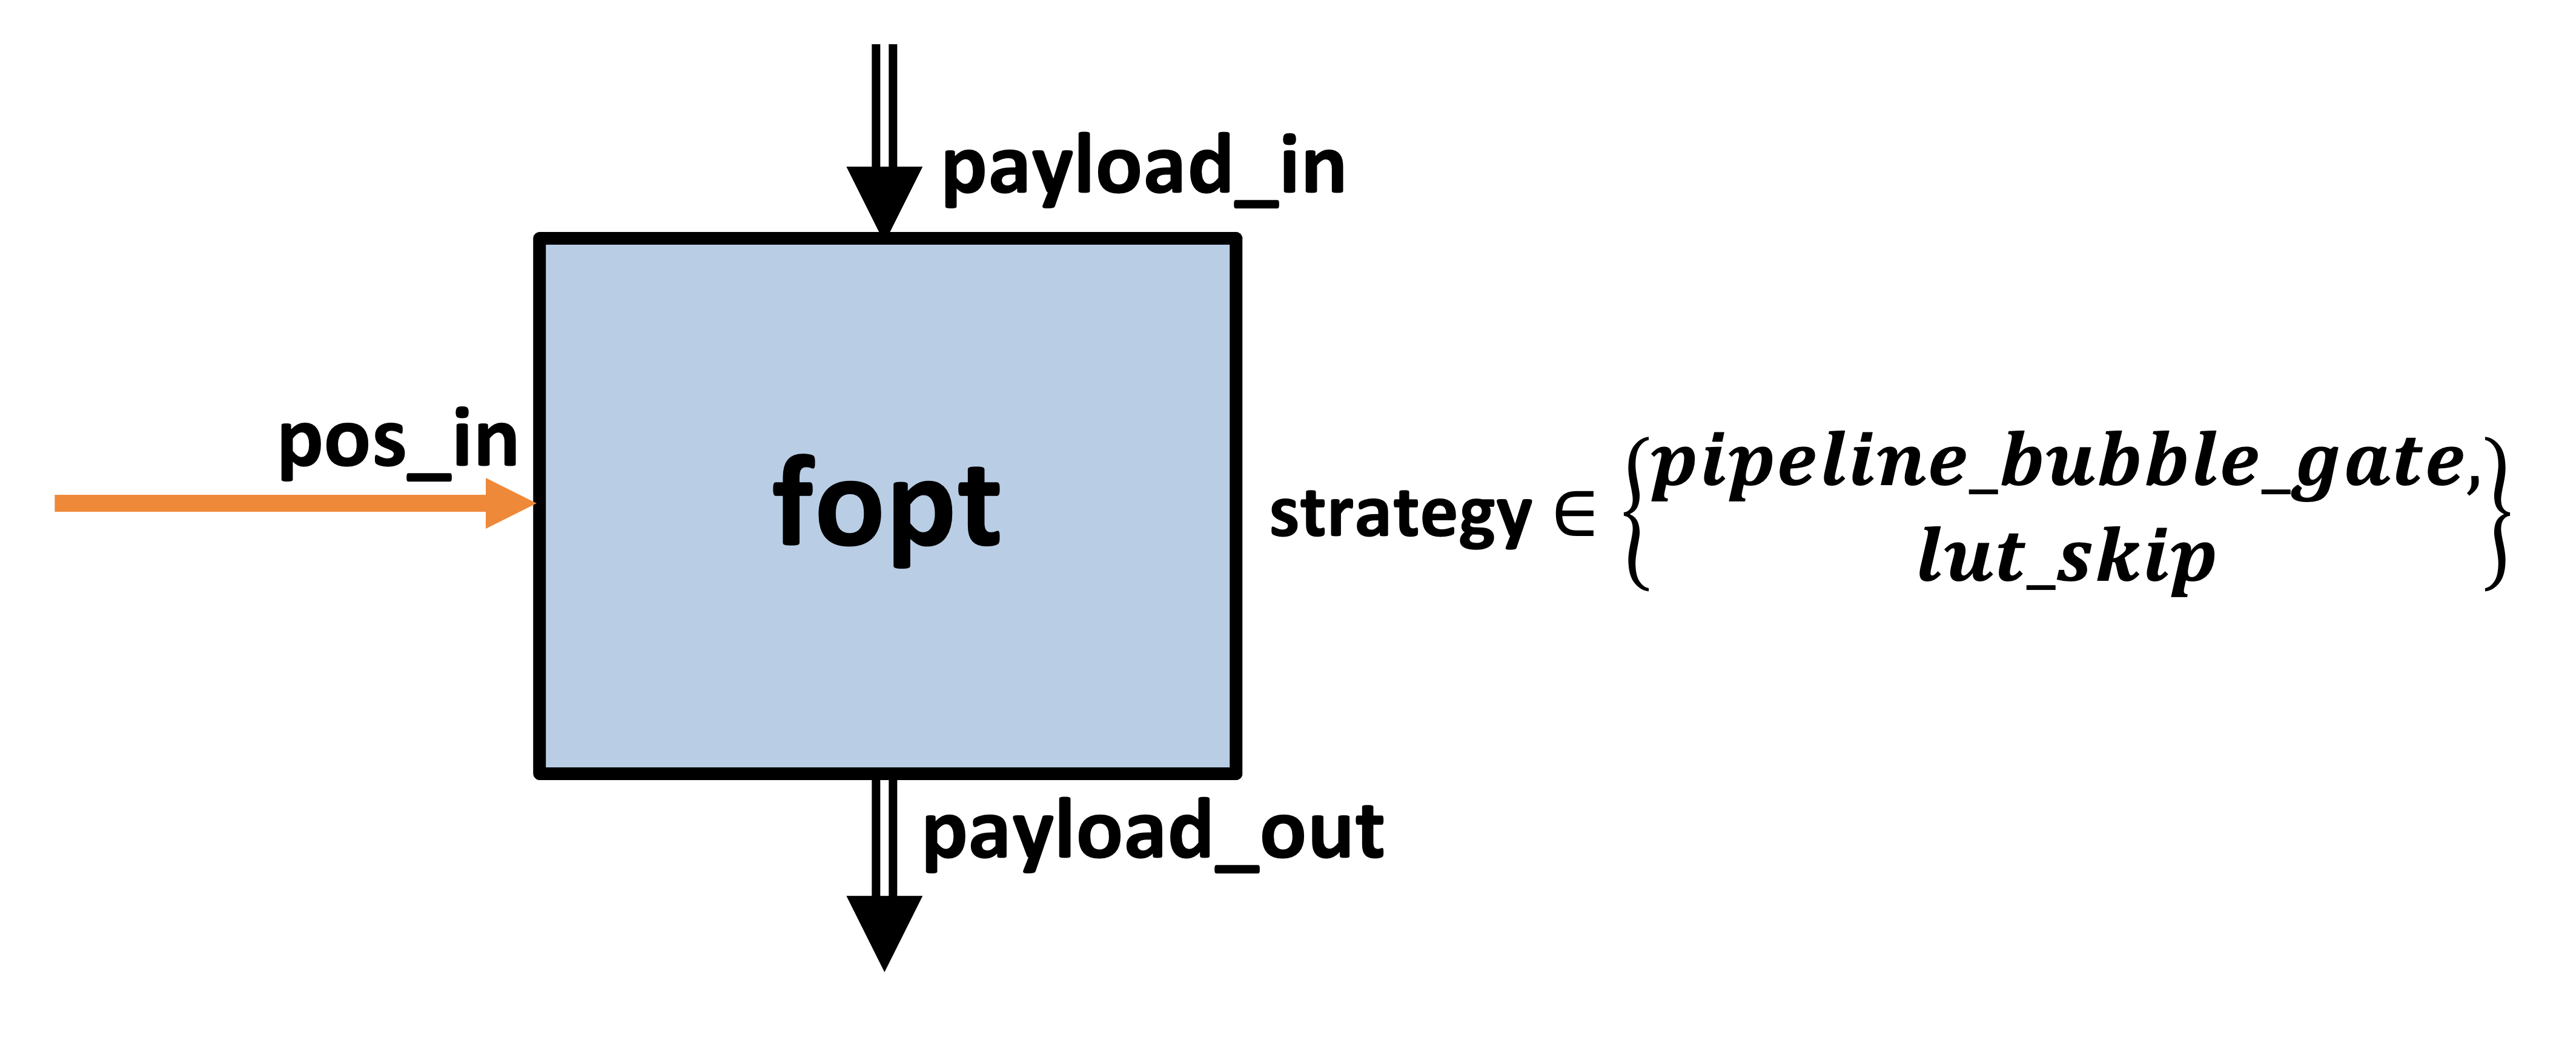
\includegraphics[width=0.95\textwidth]{figures/fopt.png}
    \caption{Fill optimizer primitive component template. }
    \label{fig:fopt}
\end{figure}

The attributes of a Fill optimizer are:

\begin{itemize}
    \item \textbf{strategy -} The fill optimization method.
    \begin{itemize}
    \item \textbf{pipeline\_bubble\_gate -} Eyeriss v2-style\cite{eyerissv2} strategy whereby unpaired leader payloads are discarded via pipeline bubble; depending on the amount of latency hiding facilitated by the pipelining, this may behave in a more gating-like or more skipping-like fashion.
    \item \textbf{lut\_skip -} GAMMA-style\cite{gamma} strategy whereby leader payloads are stored in a LUT and random-accessed by follower operand metadata. This implicitly discards unpaired leader operands.
    \end{itemize}
\end{itemize}

The supported customizations of Fill optimizer are shown in Table~\ref{tab:FillOptimizer_specializations}.

\begin{table}[H]
\centering
\begin{tabular}{l}
\toprule
 strategy             \\
\midrule
 pipeline\_bubble\_gate \\
 lut\_skip             \\
\bottomrule
\end{tabular}
\caption{Specializations of fill optimizer}
\label{tab:FillOptimizer_specializations}
\end{table}